\documentclass[12pt]{article}
\usepackage[utf8]{inputenc}
\usepackage[portuguese]{babel}
\usepackage{amsmath, amssymb}
\usepackage{graphicx}
\usepackage[margin=2.5cm]{geometry}

\title{1ª Avaliação — Processamento Digital de Sinais}
\author{Milena Freire Britto Neves, Ana Iara Loayza Costa, José Victor Brito Costa}
\date{28/07/2026}

\begin{document}
\maketitle

\section*{Questão 1}

\subsection*{a) }

Um sinal senoidal discreto $x[n] = A\cos(\omega_0 n + \theta)$ é periódico se, e somente se,
existir $N \in \mathbb{Z}^+$ e $r \in \mathbb{Z}$ tais que:
\[
\omega_0 N = 2\pi r
\]

Para o sinal dado, $\omega_0 = \dfrac{12\pi}{5}$ e $\theta = 0$. Substituindo:
\[
\frac{12\pi}{5}N = 2\pi r \;\Rightarrow\; N = \frac{5r}{6}
\]

O menor valor inteiro de $r$ que torna $N$ inteiro é $r = 6$, resultando em:
\[
N = \frac{5 \cdot 6}{6} = 5
\]

Portanto, $x[n]$ é periódico, com período fundamental $N = 5$.

\bigskip
\noindent\textit{Gráfico comprovando a periodicidade:}

\begin{figure}[h!]
    \centering
    
\includegraphics[width=0.7\textwidth]{images/grafico_1a.png}
\end{figure}

\subsection*{b) }

\textbf{Multiplicando por 2:} $\omega_0' = \dfrac{24\pi}{5}$
\[
\frac{24\pi}{5}N = 2\pi r \;\Rightarrow\; N = \frac{5r}{12}
\]
Menor $r$ inteiro válido: $r = 12 \Rightarrow N = 5$.

 O período permanece $N = 5$, mesmo dobrando a frequência. Isso explica uma
propriedade importante dos sinais discretos: diferentemente do caso contínuo
($T = 2\pi/f$, inversamente proporcional à frequência), no caso discreto essa
relação não é garantida.

\textbf{Multiplicando por 5:} $\omega_0'' = 12\pi$
\[
12\pi N = 2\pi r \;\Rightarrow\; N = \frac{r}{6}
\]
Menor $r$ inteiro válido: $r = 6 \Rightarrow N = 1$. Como $12\pi n$ é sempre múltiplo inteiro de $2\pi$, temos $\cos(12\pi n) = 1$
para todo $n$, ou seja, o sinal se torna constante (período trivial $N=1$).

\begin{figure}[h!]
    \centering
    
\includegraphics[width=0.7\textwidth]{images/grafico_1b_x2.png}
\end{figure}

\begin{figure}[h!]
    \centering
    
\includegraphics[width=0.7\textwidth]{images/grafico_1b_x5.png}
\end{figure}

\section*{Questão 2}

Foi implementada, em Python, a função \texttt{Deslocamento\_Tempo(x, n, n0)}, que
recebe o sinal $x$, seu vetor de índices $n$ e o escalar de deslocamento $n_0$, e
retorna o vetor $y$ tal que
\[
y[n] = x[n - n_0].
\]

Como o deslocamento no tempo apenas translada o sinal ao longo do eixo $n$, sem
alterar seus valores, a função retorna as mesmas amostras de $x$; o que muda é o
eixo de índices ao qual essas amostras passam a corresponder: se $x$ está definido
sobre o vetor $n$, então $y[n] = x[n-n_0]$ está definido sobre o vetor deslocado
$n_y = n + n_0$. Dessa forma, a implementação é válida para qualquer vetor $x$,
vetor de índices $n$ e escalar $n_0$ (positivo, negativo ou nulo):

\begin{verbatim}
def Deslocamento_Tempo(x, n, n0):
    x = np.asarray(x)
    y = x.copy()
    return y
\end{verbatim}

\subsection*{Exemplo}

Como exemplo, considerou-se $x[n]$ um pulso triangular definido para
$n \in [-3, 5]$, com deslocamento $n_0 = 3$ (atraso de 3 amostras). Como
$y[n] = x[n - n_0]$, o eixo de índices correspondente a $y$ é $n_y = n + n_0$.
O gráfico abaixo mostra $x[n]$ e $y[n]$ no mesmo eixo, com legenda identificando
cada sinal.

\begin{figure}[h!]
    \centering
    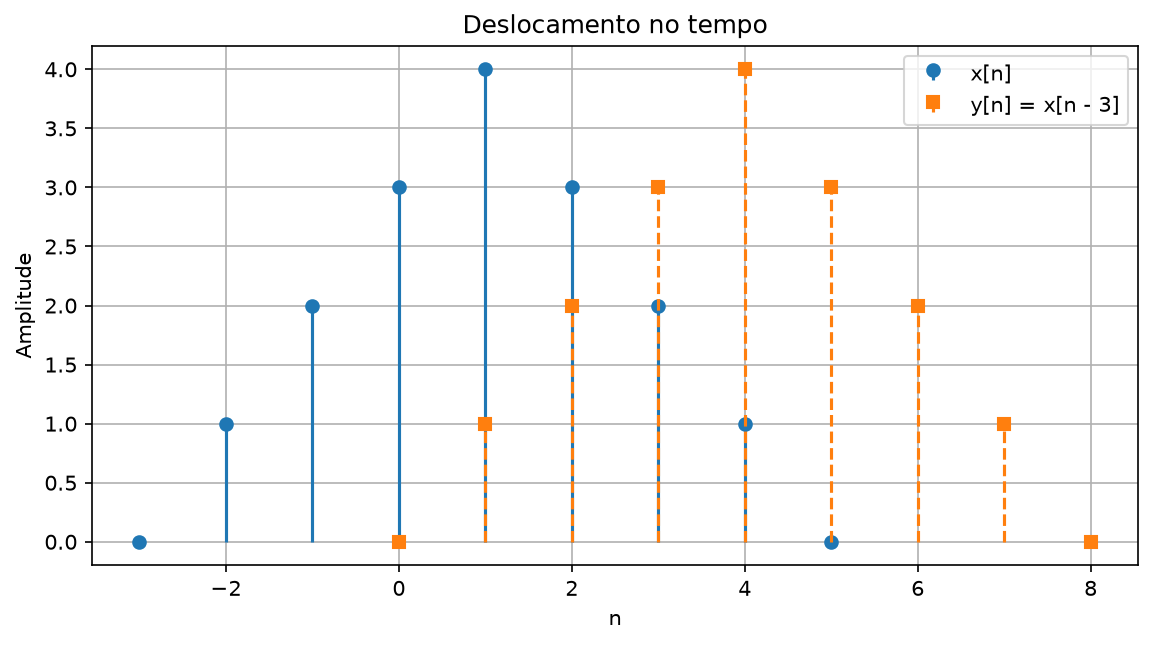
\includegraphics[width=0.7\textwidth]{images/grafico_2_deslocamento.png}
\end{figure}

\end{document}